
\documentclass[a4paper]{article}
\usepackage[utf8]{inputenc}
\usepackage{graphicx}
\usepackage{epstopdf}
\usepackage[english]{babel}
\usepackage{color}


%opening
\title{}
\author{}

\begin{document}

\maketitle

\begin{abstract}

\end{abstract}

\section{Sierra Negra experimental Set Up}
\subsection{Detector description}
\subsubsection{Small detectors}
Sierra Negra at 4550ma.s.l. is the first LAGO site with water Cherenkov detectors working (since early 2007). 
Until 2010, 3x4$m^{2}$ area Cherenkov detectors, in a 30 m triangular array were taking data at this site, 
filled with ultrapure water and covered with a reflective and diffuser material Tivek; each detector had an 
EMI 9030A photomultiplier tube, looking towards the bottom. The output of the phototube was connected to a 
data acquisition card used in the development of this fase phase 


Data Adquisition System

Field programmable gate arrays (FPGAs) was playing an increasing role in DAQ systems in cosmic rays experiments due 
to their high speed and integration and their low cost and low power consumption. Modern
electronics based on on-chip fast analog to digital converters (ADCs) and powerful digital signal processors
(DSPs) was being  ideal to be the basis of custom-made DAQ systems which are more flexible, faster and 
cheaper than the traditional DAQ systems based on modular electronics[\ref{bib:second}. We took advantage of these
recent developments, in particular in the area of very high integrated circuits in the form of ADCs and FPGAs
for the design of the new system which consisted of an ADC daughter board running at 200 MSPS. Each event
was tagged with precise GPS time using a GPS embedded receiver with 1 PPS (one pulse per second) synchronised
with the atomic clock on the GPS satellites within a corrected uncertainty of 50 ns (Motorola Oncore UT+
module). A pressure and Temperature sensor (HP03D) was adapted to the FPGA board (2FT Xilinx). A picture
of the final setup in its RF box is visible in figure \ref{sitelago0A}.


\begin{figure}[t]
\centering
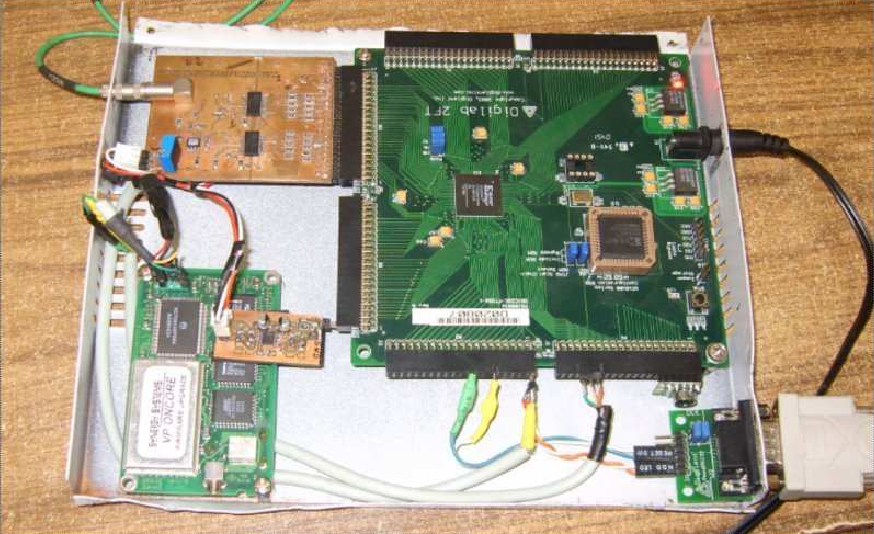
\includegraphics[scale=0.4]{/home/ruben/Documents/paperSitiosSN/paperSN0/sitelago-0A.png}
\caption{New electronics for LAGO. The prototype can be operated at 100 or 200 MSPS.}
\label{sitelago0A}
\end{figure} 




\subsubsection{Upgrade of the SN LAGO set up}

The Sierra Negra site of the LAGO experiment has four detector of 40 $m^{2}$
Three of them located at the vertex of an equilateral triangle of 30 m. 
Those detectors are cylindrical tanks, made with a corrugated steel plated
bolted with stainless steel screws, 7.3 m of diameter and 1.15 m high. The
tops and inside of each detector are covered by an EPDM (Ethylene Propylene
Diene Monomer) black liner to contain and protect the radiator media.
The EPDM material is elastic, easy to weld and mechanically very strong,
helping to have a light tight and insulated inner environment. The body and
the bottom of the detector are covered with a bag of high diffusive and
reflective material: white polyethylene banner. The white bag is filled with
high quality purified water up to a level of 1.1 m and in the upper surface;
there is a tyvek sheet floating in order to reflect the Cherenkov light
produced as uniformly as possible. The special feature of this kind of Water
Cherenkov Detector is its inner segmentation. To improve the light collection,
we have installed reflective walls with the same material that the inner liner,
The cylinder was divided at four regular sectors; one hemispherical 8 inches
diameter PMT located in the centroid of each one, looking downwards, The PMT
photocathode is submerged to avoid losses by any air-water interface. The
entire container is covered and protected externally by a black, light-tight
bag and a canvas roof. The Cherenkov light is collected by the
electron phototube 9354KB of Electron Tubes Ltd., installed up towards the 
bottom.
\begin{figure}[t]
\centering
 %\includegraphics[scale=0.5]{icrc2013-0384-01.pdf}
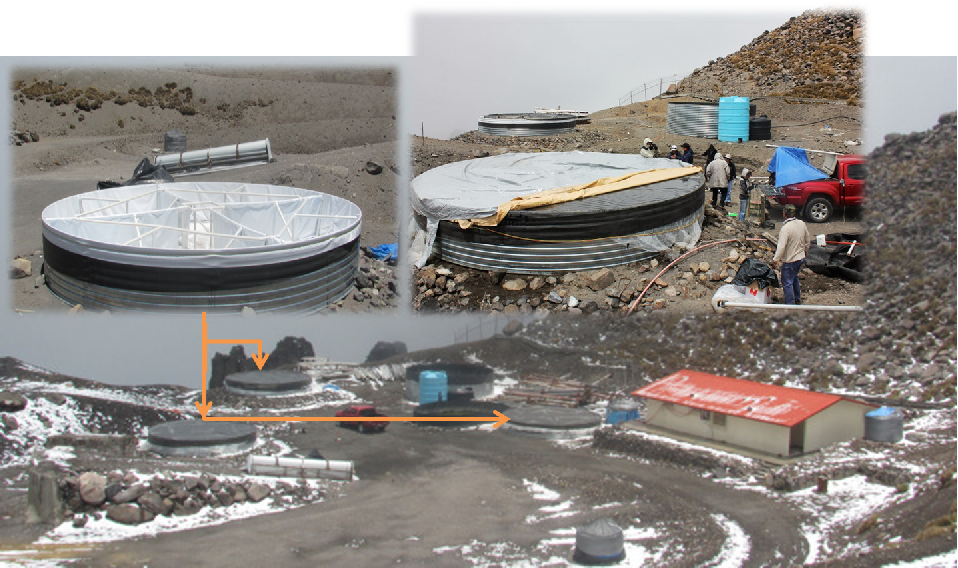
\includegraphics[scale=0.4]{/home/ruben/Documents/paperSitiosSN/paperSN0/sitelago-01.png}
\caption{LAGO Sierra Negra WCDs. An old array of small tanks is clearly seen between the new big stainless steel tanks. 
Those are covered by a black EPDM liner. B.- Internal structure of the new WCD. The structure of the PVC pipes allows us to 
set the banner walls to divide it into four sectors and fix the PMT and cables in a safety way. Also help us to keep 
the upper liner and a canvas roof.}
\label{sitelago01}
\end{figure} 

At the center of the array we will set a WCD with the same area, but  4.5m height, 
filled with clean water and with 4 Pmt at the bottom looking upwards. This detector
has the aim to reject hadrons  when  a extensive air shower is detected.

\subsection{Data Acquisition System}
The custom-made instrumentation for the DAQ system uses low power consumption,
it includes: A 4-channel ADC daughter-board with two dual 10-bit ADC chip
from Analog Devices, this chip was the AD9216 that is a dual, 3 V, 10-bit,
105 MSPS analog-to-digital converter. The daughter-board is connected to a
second board with an FPGA, for real-time data processing (Nexys2 from Digilent
Inc.); This board is a powerful digital system design platform built around a
Xilinx Spartan 3E FPGA, with 16 Mb of fast SDRAM and 16 Mb of Flash ROM. The
Nexys2 board is ideally suited to embedded processors like Xilinx's 32-bit
RISC Microblaze. Communication and control are based on a small minicomputer
Raspberry PI model B 512MB with an ARM1176JZF-S 700 MHz processor, this mini-
computer is the main control between the host y the DAQ, and it is used for
interconnection with the surface detector modules, the mother board has two
ways of communication with the host, the first one uses a serial port with a
typical communication rate around 115200 bits per second and the second one
uses a USB port with a higher communication speed.

A pressure and temperature sensor, (HP03D from Shenzhen Hope Microelectronics
Co. Ltd.) which includes a piezo-resistive pressure sensor and an ADC interface,
providing 16 bit word data for pressure and temperature related voltage, is
connected to the FPGA board. The algorithms developed use advanced digital
signal processing techniques and particularly digital pulse processing, where
the purpose of the pulse processing is to perform on-line signal processing
on the digitized signals directly to minimize the data transfer size, these
algorithms are implemented on the FPGA using Hardware Description Language
(VHDL) and C Language for the Microblaze processor, these algorithms can be
reprogrammed at any time. Each event is tagged with precise GPS time tags using
an embedded GPS receiver with 1 PPS (one pulse per second) synchronized with
UTC within an uncertainty of 50 ns (Motorola Oncore UT+ GPS receiver), see figure \ref{sitelago02}
and figure \ref{sitelago03}. The bitstream firmware of the DAQ system resides permanently on the
Flash ROM chip located on the mother board and it gets downloaded into the FPGA
upon power on. On the PC side we use Perl and Python under Linux to process,
store and display the data acquired. Finally, we use ROOT programs to histogram
and analyze the data.

\begin{figure}[t]
\centering
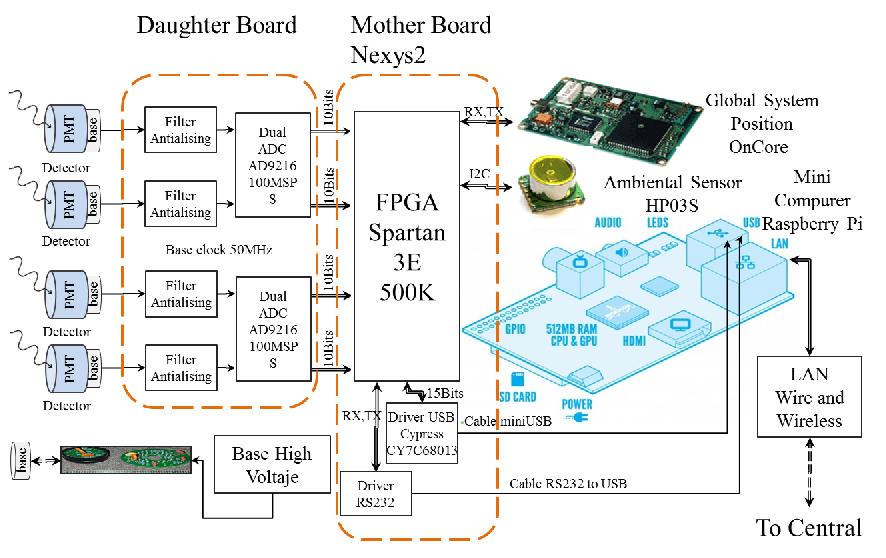
\includegraphics[scale=0.5]{/home/ruben/Documents/paperSitiosSN/paperSN0/sitelago-02.png}
\caption{DAQ full blocks diagram, you can see the main parts of the DAQ.1.- Daughter Board 2.- Mother Board, and 3.- Host.}
\label{sitelago02}
\end{figure} 

\begin{figure}[t]
\centering
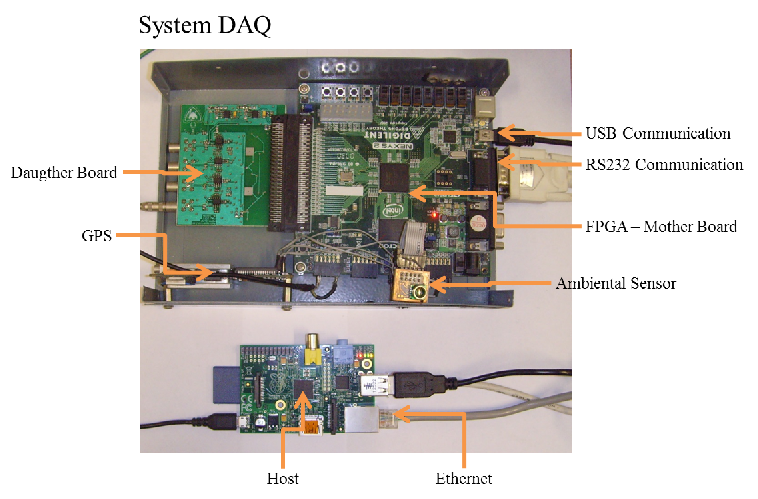
\includegraphics[scale=0.5]{/home/ruben/Documents/paperSitiosSN/paperSN0/sitelago-03.png}
\caption{A view of the custom electronics used at LAGO.}
\label{sitelago03}
\end{figure} 

%% ====================================================
\section{Operation and calibration of the WCD Detectors}
%2.-Operation and calibration of the WCD Detectors.

Calibration mode. It consists on the data acquisition of 32 consecutive samples
in 10 ns intervals (100MSPS) of the digital pulses produced by an ultraviolet
LED with wavelength of 405 nm with a 15 ns wide pulse in a frequency of 10kHz
located 60 cm from the PMT. The phototube polarization voltage and the LED
polarization voltage are fine tuned. It provides us with a minimal response
that represents a fundamental part for the calibration of a PMT.

As shown in figure \ref{sitelago04} and figure, \ref{sitelago05},we can plot the response to a single photo-electron using
our DAQ. The curves correspond to high voltages of 1.25 kV, 1.3 kV,
and 1.35 kV. The best single photo-electron response, for this PMT, is obtained
at 1.3 kV and this value was set as the operation one.
 

\begin{figure}[t]
\centering
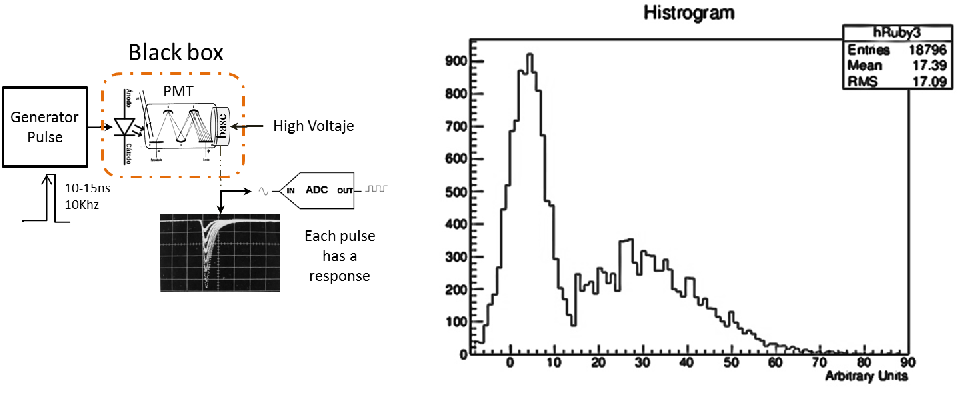
\includegraphics[scale=0.4]{/home/ruben/Documents/paperSitiosSN/paperSN0/sitelago-04.png}
\caption{Mode calibration and Response to a single photo-electron, using the new DAQ.}
\label{sitelago04}
\end{figure} 

\begin{figure}[t]
\centering
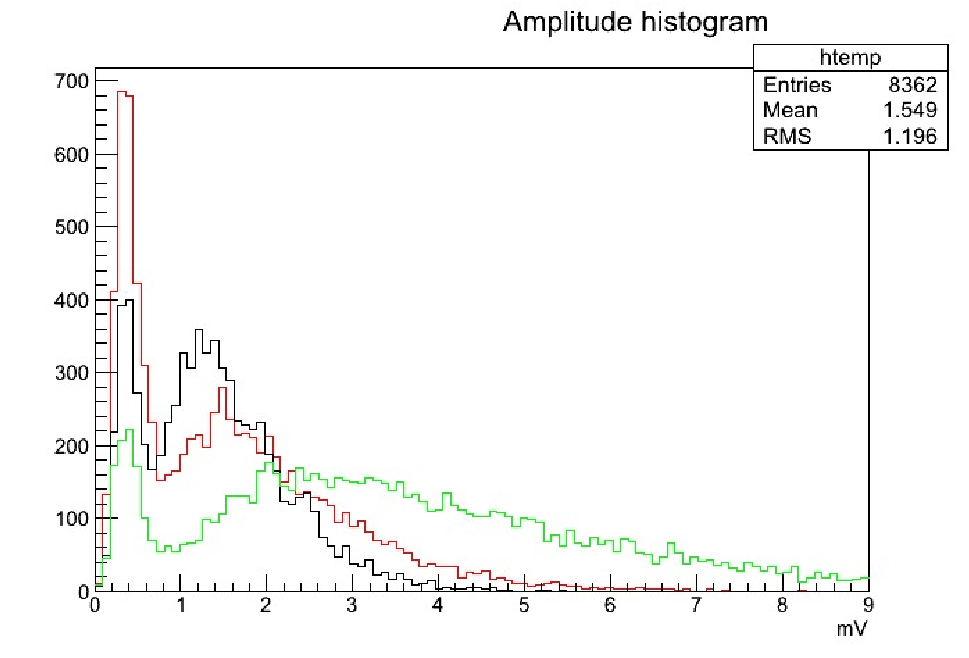
\includegraphics[scale=0.4]{/home/ruben/Documents/paperSitiosSN/paperSN0/sitelago-05.png}
\caption{Plot of the response to a single photo-electron by the PMT at 1.25 kV (black), 1.3 kV (red), and 1.35 kV (green). The operation voltage was fixed at 1.3 kV.}
\label{sitelago05}
\end{figure} 


Examples of traces, baseline and threshold are shown in \textcolor{red}{\ref{sitelago06}}

\begin{figure}[t]
\centering
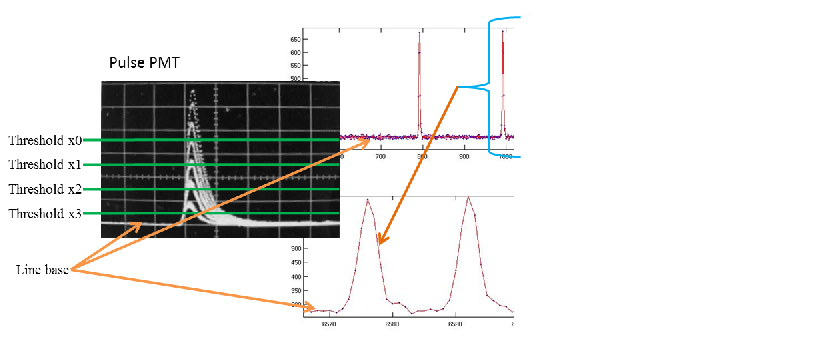
\includegraphics[scale=0.5]{/home/ruben/Documents/paperSitiosSN/paperSN0/sitelago-06.png}
\caption{Example who shows the basic line, trace, rate.}
\label{sitelago06}
\end{figure} 

Sites Located at the Sierra Negra site (4550 m.a.s.l) in the State of Puebla, México.
$18^o 59^{"}$, $97^o  18^{"}$ Magnetic rigidity cutoff 9 GV.

%% ====================================================

\begin{thebibliography}{}
\bibitem{bib:lattes} Pierre Auger Collaboration, 2004, NIM A 523, 50-95
\bibitem{bib:second}D. Allard, C. Alvarez, H. Asorey et. al. "Operating Water Cherenkov Detectors in high altitude sites for the
Large Aperture GRB Observatory", sec IV, Proceedings of the 31st ICRC, ŁODZ 2009.
\bibitem{bib:third}Conde Sanchez Rubén for the LAGO Collaboration,  "The Upgrade of the LAGO Project at Sierra Negra, México", Proceedings of the 33rd ICRC, Rio de Janerio 2013.
\bibitem{bib:four}A. Sandoval for the  HAWC Collaboration, "A Third Generation Water Cherenkov Observatory", Proceedings of the 33rd ICRC, Rio de Janerio 2013.
\end{thebibliography}


\end{document}

